\documentclass{article}
\usepackage{graphicx}
\usepackage{tikz}
\usepackage[cm]{fullpage}
\usepackage{amssymb,amsmath}
\usepackage{natbib}
\DeclareMathOperator*{\argmin}{arg\,min}
\DeclareMathOperator*{\sign}{sign}
\DeclareMathOperator*{\Lik}{Lik}
\DeclareMathOperator*{\Peaks}{Peaks}
\DeclareMathOperator*{\HotSpots}{HotSpots}
\newcommand{\Cost}{\text{Cost}}
\usepackage{stfloats}
\DeclareMathOperator*{\Diag}{Diag}
\DeclareMathOperator*{\TPR}{TPR}
\DeclareMathOperator*{\Segments}{Segments}
\DeclareMathOperator*{\Changes}{Changes}
\DeclareMathOperator*{\FPR}{FPR}
\DeclareMathOperator*{\argmax}{arg\,max}
\DeclareMathOperator*{\maximize}{maximize}
\DeclareMathOperator*{\minimize}{minimize}
\newcommand{\ZZ}{\mathbb Z}
\newcommand{\NN}{\mathbb N}
\newcommand{\RR}{\mathbb R}

\begin{document}

\title{A linear time algorithm for peak detection using constrained
  optimal segmentation}

\author{Toby Dylan Hocking and Guillem Rigaill}

\maketitle

\section{Introduction}

\citet{FPOP} proposed the Functional Pruning Optimal Partitioning
(FPOP) Algorithm to exactly solve the penalized segmentation
problem. In this paper we use the FPOP algorithm to solve the
penalized version of the PeakSeg problem \citep{PeakSeg}.

\section{Problem setting}

\subsection{Unconstrained model}

We have a genomic data set $\mathbf{z}\in\ZZ_+^B$ of counts on $B$
bases. The unconstrained problem for a positive penalty parameter
$\lambda\in\RR_+$ is
\begin{equation}
  \label{unconstrained}
  \mathbf{\hat m}^\lambda(\mathbf z)  =\ 
  \argmin_{\mathbf m\in\RR^{B}}\ 
  \rho
  %\tag{\textbf{Unconstrained}}
  (\mathbf m, \mathbf z) 
  +\lambda\Changes(\mathbf m),
\end{equation}
where the Poisson loss function is
\begin{equation}\label{eq:rho}
  \rho(\mathbf m, \mathbf z)= \sum_{b=1}^B m_b - z_b \log m_b.
\end{equation} 
The model complexity is the number of change-points
\begin{equation}
  \Changes(\mathbf m)=\sum_{b=2}^B I(m_{b-1} \neq m_b),
\end{equation}
where $I$ is the indicator function.

Although it is a non-convex optimization problem, the segmentation
$\mathbf{\hat m}^\lambda(\mathbf z)$ can be computed in linear $O(B)$
time using the FPOP algorithm \citep{FPOP}.

We refer to (\ref{unconstrained}) as the ``unconstrained'' model since
$\mathbf{\hat m}^\lambda(\mathbf z)$ can have any sequence of changes
up or down. However for the purposes of peak detection, we are only
interested in segmentations with alternating changes that can be
interpreted as peaks and background \citep{PeakSeg}.

More concretely, we first define the peak indicator at base
$b\in\{2, \dots, B\}$ as
\begin{equation}
  \label{eq:peaks}
  P_b(\mathbf m) = \sum_{j=2}^b \sign( m_{j} - m_{j-1} ),
\end{equation}
where $P_1(\mathbf m)=0$ by convention. $P_b(\mathbf m)$ is the
cumulative sum of signs of changes up to point $b$ in the piecewise
constant vector $\mathbf m$. We define the vector of peak indicators
as
\begin{equation}
  \mathbf
  P[\mathbf m] = \left[
    \begin{array}{ccc}
      P_1(\mathbf m) & \cdots & P_B(\mathbf m)
    \end{array}\right].
\end{equation}

\subsection{PenPeakSeg: penalized constrained segmentation}
\label{sec:constrained}

In general for the unconstrained model $P_b(\mathbf m)\in\ZZ$, which
is problematic since we want to use it as a peak detector with binary
outputs $P_b(\mathbf m)\in \{0, 1\}$. 
For example, if $\mathbf m = \left[\begin{array}{ccccccc}1.1 &
    1.1 & 2 & 2 & 4 & 4 & 3\end{array}\right]$, with two changes up
followed by one change down, then $\mathbf P(\mathbf m) =
\left[\begin{array}{ccccccc}0 & 0 & 1 & 1 & 2 & 2 &
    1 \end{array}\right]$.
Thus we constrain the peak indicator $P_b(\mathbf m)\in\{0, 1\}$,
which results in the constrained problem
\begin{align*}
  \label{PenPeakSeg}
  \mathbf{\tilde m}^\lambda(\mathbf z)  =
  \argmin_{\mathbf m\in\RR^{B}} &\ \ 
    \rho(\mathbf m, \mathbf z) + \lambda\Peaks(\mathbf m)
    \tag{\textbf{PenPeakSeg}}
  \\
  \text{such that} &\ \forall b\in\{1, \dots, B\},
                     \ \ P_b(\mathbf m) \in\{0, 1\}.
\end{align*}
The Peaks model complexity term only counts up changes:
\begin{equation}
  \Peaks(\mathbf m) = \sum_{b=2}^B I(m_{b-1} < m_b).
\end{equation}
The constraint in the \ref{PenPeakSeg} problem forces the sequence of
changes in the segment means $\mathbf m$ to begin with a positive
change and then alternate: up, down, up, down, ... (and not up, up,
down). Thus the even-numbered segments may be interpreted as peaks
$P_b(\mathbf m)=1$, and the odd-numbered segments may be interpreted
as background $P_b(\mathbf m)=0$.

\section{Algorithm}

\subsection{Segment Neighborhood}

For the Segment Neighborhood algorithm we begin as usual by computing
a functional representation of the optimal cost in 1 segment up to
base $b$. 
\begin{equation*}
  \label{eq:C1b}
  C_{1,b}(\mu) = \sum_{i=1}^b \gamma_b(\mu),
\end{equation*}
where $\gamma_b(\mu)$ is the cost of using the mean $\mu$ for single
data point $b$ (for example the Gaussian or Poisson loss).

Next we define the minimum cost in 2 segments up to data point 2 as
\begin{equation*}
  \label{eq:C22}
  C_{2,2}(\mu) = C_{1,1}^{\leq}(\mu) + \gamma_2(\mu),
\end{equation*}
where for a function $f:\RR\rightarrow\RR$ the min-less operator
yields another function $f\leq:\RR\rightarrow\RR$ such that
\begin{equation}
  \label{eq:min-less}
  f^{\leq}(\mu) = \min_{x\leq \mu} f(x).
\end{equation}
The algorithm relies on the ability to compute an exact representation
of functions such as $C_{1,1}^{\leq}$. Since the cost functions $f$
are quasiconvex, we can easily find the minimum $\mu^*$, and then
compute the following exact representation
\begin{equation*}
  f^\leq(\mu)
  \begin{cases}
    f(\mu^*) & \text{ if } \mu \geq \mu^*,\\
    f(\mu) & \text{ otherwise.}
  \end{cases}
\end{equation*}

\begin{center}
  % Created by tikzDevice version 0.9 on 2016-05-03 17:46:56
% !TEX encoding = UTF-8 Unicode
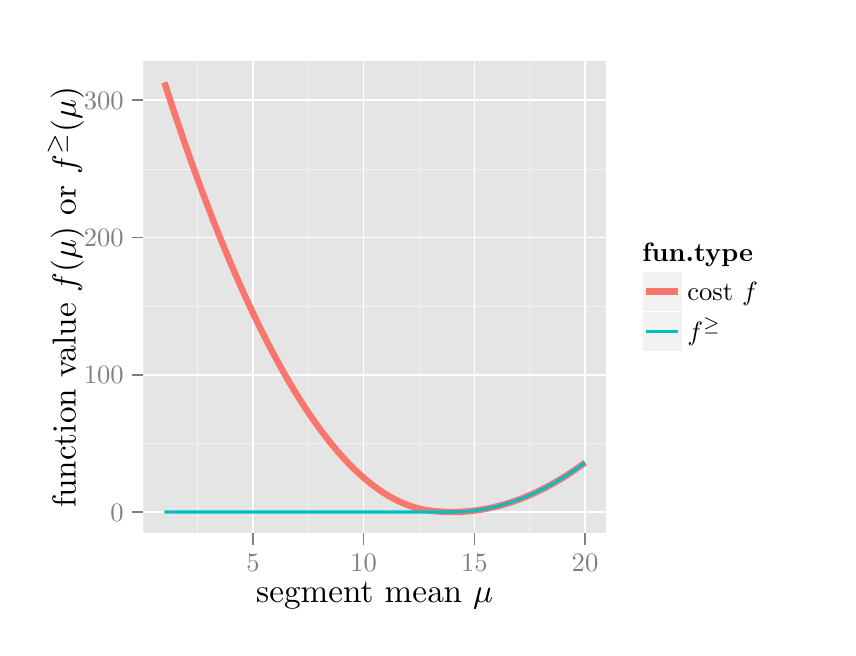
\begin{tikzpicture}[x=1pt,y=1pt]
\definecolor{fillColor}{RGB}{255,255,255}
\path[use as bounding box,fill=fillColor,fill opacity=0.00] (0,0) rectangle (289.08,216.81);
\begin{scope}
\path[clip] (  0.00,  0.00) rectangle (289.08,216.81);
\definecolor{drawColor}{RGB}{255,255,255}
\definecolor{fillColor}{RGB}{255,255,255}

\path[draw=drawColor,line width= 0.6pt,line join=round,line cap=round,fill=fillColor] ( -0.00,  0.00) rectangle (289.08,216.81);
\end{scope}
\begin{scope}
\path[clip] ( 41.82, 34.03) rectangle (208.99,204.77);
\definecolor{fillColor}{gray}{0.90}

\path[fill=fillColor] ( 41.82, 34.03) rectangle (208.99,204.76);
\definecolor{drawColor}{gray}{0.95}

\path[draw=drawColor,line width= 0.3pt,line join=round] ( 41.82, 66.59) --
	(208.99, 66.59);

\path[draw=drawColor,line width= 0.3pt,line join=round] ( 41.82,116.18) --
	(208.99,116.18);

\path[draw=drawColor,line width= 0.3pt,line join=round] ( 41.82,165.76) --
	(208.99,165.76);

\path[draw=drawColor,line width= 0.3pt,line join=round] ( 61.42, 34.03) --
	( 61.42,204.77);

\path[draw=drawColor,line width= 0.3pt,line join=round] (101.41, 34.03) --
	(101.41,204.77);

\path[draw=drawColor,line width= 0.3pt,line join=round] (141.40, 34.03) --
	(141.40,204.77);

\path[draw=drawColor,line width= 0.3pt,line join=round] (181.39, 34.03) --
	(181.39,204.77);
\definecolor{drawColor}{RGB}{255,255,255}

\path[draw=drawColor,line width= 0.6pt,line join=round] ( 41.82, 41.80) --
	(208.99, 41.80);

\path[draw=drawColor,line width= 0.6pt,line join=round] ( 41.82, 91.38) --
	(208.99, 91.38);

\path[draw=drawColor,line width= 0.6pt,line join=round] ( 41.82,140.97) --
	(208.99,140.97);

\path[draw=drawColor,line width= 0.6pt,line join=round] ( 41.82,190.56) --
	(208.99,190.56);

\path[draw=drawColor,line width= 0.6pt,line join=round] ( 81.41, 34.03) --
	( 81.41,204.77);

\path[draw=drawColor,line width= 0.6pt,line join=round] (121.40, 34.03) --
	(121.40,204.77);

\path[draw=drawColor,line width= 0.6pt,line join=round] (161.40, 34.03) --
	(161.40,204.77);

\path[draw=drawColor,line width= 0.6pt,line join=round] (201.39, 34.03) --
	(201.39,204.77);
\definecolor{drawColor}{RGB}{248,118,109}

\path[draw=drawColor,line width= 2.3pt,line join=round] ( 49.42,197.00) --
	( 50.39,194.01) --
	( 51.36,191.05) --
	( 52.33,188.12) --
	( 53.30,185.22) --
	( 54.27,182.34) --
	( 55.24,179.50) --
	( 56.20,176.68) --
	( 57.17,173.89) --
	( 58.14,171.14) --
	( 59.11,168.41) --
	( 60.08,165.71) --
	( 61.05,163.04) --
	( 62.02,160.40) --
	( 62.99,157.79) --
	( 63.96,155.20) --
	( 64.93,152.65) --
	( 65.90,150.13) --
	( 66.87,147.63) --
	( 67.84,145.16) --
	( 68.81,142.73) --
	( 69.78,140.32) --
	( 70.75,137.94) --
	( 71.72,135.59) --
	( 72.69,133.27) --
	( 73.66,130.98) --
	( 74.63,128.72) --
	( 75.59,126.48) --
	( 76.56,124.28) --
	( 77.53,122.10) --
	( 78.50,119.96) --
	( 79.47,117.84) --
	( 80.44,115.76) --
	( 81.41,113.70) --
	( 82.38,111.67) --
	( 83.35,109.67) --
	( 84.32,107.70) --
	( 85.29,105.76) --
	( 86.26,103.84) --
	( 87.23,101.96) --
	( 88.20,100.11) --
	( 89.17, 98.28) --
	( 90.14, 96.48) --
	( 91.11, 94.72) --
	( 92.08, 92.98) --
	( 93.05, 91.27) --
	( 94.02, 89.59) --
	( 94.99, 87.94) --
	( 95.95, 86.32) --
	( 96.92, 84.73) --
	( 97.89, 83.17) --
	( 98.86, 81.63) --
	( 99.83, 80.13) --
	(100.80, 78.65) --
	(101.77, 77.21) --
	(102.74, 75.79) --
	(103.71, 74.40) --
	(104.68, 73.04) --
	(105.65, 71.71) --
	(106.62, 70.41) --
	(107.59, 69.14) --
	(108.56, 67.90) --
	(109.53, 66.69) --
	(110.50, 65.50) --
	(111.47, 64.35) --
	(112.44, 63.22) --
	(113.41, 62.13) --
	(114.38, 61.06) --
	(115.34, 60.02) --
	(116.31, 59.01) --
	(117.28, 58.03) --
	(118.25, 57.08) --
	(119.22, 56.16) --
	(120.19, 55.27) --
	(121.16, 54.40) --
	(122.13, 53.57) --
	(123.10, 52.76) --
	(124.07, 51.99) --
	(125.04, 51.24) --
	(126.01, 50.52) --
	(126.98, 49.84) --
	(127.95, 49.18) --
	(128.92, 48.55) --
	(129.89, 47.94) --
	(130.86, 47.37) --
	(131.83, 46.83) --
	(132.80, 46.32) --
	(133.77, 45.83) --
	(134.73, 45.38) --
	(135.70, 44.95) --
	(136.67, 44.55) --
	(137.64, 44.19) --
	(138.61, 43.85) --
	(139.58, 43.54) --
	(140.55, 43.26) --
	(141.52, 43.00) --
	(142.49, 42.78) --
	(143.46, 42.59) --
	(144.43, 42.43) --
	(145.40, 42.29) --
	(145.40, 42.29) --
	(145.97, 42.22) --
	(146.53, 42.16) --
	(147.10, 42.10) --
	(147.66, 42.05) --
	(148.23, 42.00) --
	(148.79, 41.96) --
	(149.36, 41.92) --
	(149.92, 41.89) --
	(150.49, 41.86) --
	(151.06, 41.84) --
	(151.62, 41.82) --
	(152.19, 41.81) --
	(152.75, 41.80) --
	(153.32, 41.80) --
	(153.88, 41.80) --
	(154.45, 41.80) --
	(155.01, 41.82) --
	(155.58, 41.83) --
	(156.15, 41.85) --
	(156.71, 41.88) --
	(157.28, 41.91) --
	(157.84, 41.95) --
	(158.41, 41.99) --
	(158.97, 42.04) --
	(159.54, 42.09) --
	(160.10, 42.14) --
	(160.67, 42.20) --
	(161.23, 42.27) --
	(161.80, 42.34) --
	(162.37, 42.42) --
	(162.93, 42.50) --
	(163.50, 42.59) --
	(164.06, 42.68) --
	(164.63, 42.77) --
	(165.19, 42.87) --
	(165.76, 42.98) --
	(166.32, 43.09) --
	(166.89, 43.21) --
	(167.46, 43.33) --
	(168.02, 43.45) --
	(168.59, 43.58) --
	(169.15, 43.72) --
	(169.72, 43.86) --
	(170.28, 44.01) --
	(170.85, 44.16) --
	(171.41, 44.31) --
	(171.98, 44.47) --
	(172.55, 44.64) --
	(173.11, 44.81) --
	(173.68, 44.98) --
	(174.24, 45.16) --
	(174.81, 45.35) --
	(175.37, 45.54) --
	(175.94, 45.73) --
	(176.50, 45.93) --
	(177.07, 46.14) --
	(177.64, 46.35) --
	(178.20, 46.56) --
	(178.77, 46.78) --
	(179.33, 47.01) --
	(179.90, 47.24) --
	(180.46, 47.47) --
	(181.03, 47.71) --
	(181.59, 47.96) --
	(182.16, 48.21) --
	(182.73, 48.46) --
	(183.29, 48.72) --
	(183.86, 48.99) --
	(184.42, 49.26) --
	(184.99, 49.53) --
	(185.55, 49.81) --
	(186.12, 50.09) --
	(186.68, 50.38) --
	(187.25, 50.68) --
	(187.82, 50.98) --
	(188.38, 51.28) --
	(188.95, 51.59) --
	(189.51, 51.90) --
	(190.08, 52.22) --
	(190.64, 52.55) --
	(191.21, 52.88) --
	(191.77, 53.21) --
	(192.34, 53.55) --
	(192.91, 53.89) --
	(193.47, 54.24) --
	(194.04, 54.60) --
	(194.60, 54.95) --
	(195.17, 55.32) --
	(195.73, 55.69) --
	(196.30, 56.06) --
	(196.86, 56.44) --
	(197.43, 56.82) --
	(198.00, 57.21) --
	(198.56, 57.60) --
	(199.13, 58.00) --
	(199.69, 58.41) --
	(200.26, 58.82) --
	(200.82, 59.23) --
	(201.39, 59.65);
\definecolor{drawColor}{RGB}{0,191,196}

\path[draw=drawColor,line width= 1.1pt,line join=round] ( 49.42, 41.80) --
	( 50.47, 41.80) --
	( 51.52, 41.80) --
	( 52.57, 41.80) --
	( 53.62, 41.80) --
	( 54.67, 41.80) --
	( 55.72, 41.80) --
	( 56.77, 41.80) --
	( 57.82, 41.80) --
	( 58.87, 41.80) --
	( 59.92, 41.80) --
	( 60.97, 41.80) --
	( 62.02, 41.80) --
	( 63.07, 41.80) --
	( 64.12, 41.80) --
	( 65.17, 41.80) --
	( 66.22, 41.80) --
	( 67.27, 41.80) --
	( 68.32, 41.80) --
	( 69.37, 41.80) --
	( 70.42, 41.80) --
	( 71.47, 41.80) --
	( 72.52, 41.80) --
	( 73.57, 41.80) --
	( 74.63, 41.80) --
	( 75.68, 41.80) --
	( 76.73, 41.80) --
	( 77.78, 41.80) --
	( 78.83, 41.80) --
	( 79.88, 41.80) --
	( 80.93, 41.80) --
	( 81.98, 41.80) --
	( 83.03, 41.80) --
	( 84.08, 41.80) --
	( 85.13, 41.80) --
	( 86.18, 41.80) --
	( 87.23, 41.80) --
	( 88.28, 41.80) --
	( 89.33, 41.80) --
	( 90.38, 41.80) --
	( 91.43, 41.80) --
	( 92.48, 41.80) --
	( 93.53, 41.80) --
	( 94.58, 41.80) --
	( 95.63, 41.80) --
	( 96.68, 41.80) --
	( 97.73, 41.80) --
	( 98.78, 41.80) --
	( 99.83, 41.80) --
	(100.88, 41.80) --
	(101.93, 41.80) --
	(102.98, 41.80) --
	(104.03, 41.80) --
	(105.08, 41.80) --
	(106.13, 41.80) --
	(107.18, 41.80) --
	(108.23, 41.80) --
	(109.29, 41.80) --
	(110.34, 41.80) --
	(111.39, 41.80) --
	(112.44, 41.80) --
	(113.49, 41.80) --
	(114.54, 41.80) --
	(115.59, 41.80) --
	(116.64, 41.80) --
	(117.69, 41.80) --
	(118.74, 41.80) --
	(119.79, 41.80) --
	(120.84, 41.80) --
	(121.89, 41.80) --
	(122.94, 41.80) --
	(123.99, 41.80) --
	(125.04, 41.80) --
	(126.09, 41.80) --
	(127.14, 41.80) --
	(128.19, 41.80) --
	(129.24, 41.80) --
	(130.29, 41.80) --
	(131.34, 41.80) --
	(132.39, 41.80) --
	(133.44, 41.80) --
	(134.49, 41.80) --
	(135.54, 41.80) --
	(136.59, 41.80) --
	(137.64, 41.80) --
	(138.69, 41.80) --
	(139.74, 41.80) --
	(140.79, 41.80) --
	(141.84, 41.80) --
	(142.90, 41.80) --
	(143.95, 41.80) --
	(145.00, 41.80) --
	(146.05, 41.80) --
	(147.10, 41.80) --
	(148.15, 41.80) --
	(149.20, 41.80) --
	(150.25, 41.80) --
	(151.30, 41.80) --
	(152.35, 41.80) --
	(153.40, 41.80) --
	(153.40, 41.80) --
	(153.88, 41.80) --
	(154.37, 41.80) --
	(154.85, 41.81) --
	(155.34, 41.82) --
	(155.82, 41.84) --
	(156.31, 41.86) --
	(156.79, 41.88) --
	(157.28, 41.91) --
	(157.76, 41.94) --
	(158.25, 41.98) --
	(158.73, 42.02) --
	(159.22, 42.06) --
	(159.70, 42.10) --
	(160.18, 42.15) --
	(160.67, 42.20) --
	(161.15, 42.26) --
	(161.64, 42.32) --
	(162.12, 42.39) --
	(162.61, 42.45) --
	(163.09, 42.52) --
	(163.58, 42.60) --
	(164.06, 42.68) --
	(164.55, 42.76) --
	(165.03, 42.84) --
	(165.52, 42.93) --
	(166.00, 43.03) --
	(166.49, 43.12) --
	(166.97, 43.22) --
	(167.46, 43.33) --
	(167.94, 43.43) --
	(168.43, 43.55) --
	(168.91, 43.66) --
	(169.40, 43.78) --
	(169.88, 43.90) --
	(170.36, 44.03) --
	(170.85, 44.16) --
	(171.33, 44.29) --
	(171.82, 44.43) --
	(172.30, 44.57) --
	(172.79, 44.71) --
	(173.27, 44.86) --
	(173.76, 45.01) --
	(174.24, 45.16) --
	(174.73, 45.32) --
	(175.21, 45.48) --
	(175.70, 45.65) --
	(176.18, 45.82) --
	(176.67, 45.99) --
	(177.15, 46.17) --
	(177.64, 46.35) --
	(178.12, 46.53) --
	(178.61, 46.72) --
	(179.09, 46.91) --
	(179.57, 47.11) --
	(180.06, 47.30) --
	(180.54, 47.51) --
	(181.03, 47.71) --
	(181.51, 47.92) --
	(182.00, 48.14) --
	(182.48, 48.35) --
	(182.97, 48.57) --
	(183.45, 48.80) --
	(183.94, 49.02) --
	(184.42, 49.26) --
	(184.91, 49.49) --
	(185.39, 49.73) --
	(185.88, 49.97) --
	(186.36, 50.22) --
	(186.85, 50.47) --
	(187.33, 50.72) --
	(187.82, 50.98) --
	(188.30, 51.24) --
	(188.79, 51.50) --
	(189.27, 51.77) --
	(189.75, 52.04) --
	(190.24, 52.32) --
	(190.72, 52.59) --
	(191.21, 52.88) --
	(191.69, 53.16) --
	(192.18, 53.45) --
	(192.66, 53.75) --
	(193.15, 54.04) --
	(193.63, 54.34) --
	(194.12, 54.65) --
	(194.60, 54.95) --
	(195.09, 55.27) --
	(195.57, 55.58) --
	(196.06, 55.90) --
	(196.54, 56.22) --
	(197.03, 56.55) --
	(197.51, 56.88) --
	(198.00, 57.21) --
	(198.48, 57.55) --
	(198.97, 57.89) --
	(199.45, 58.23) --
	(199.93, 58.58) --
	(200.42, 58.93) --
	(200.90, 59.29) --
	(201.39, 59.65);
\end{scope}
\begin{scope}
\path[clip] (  0.00,  0.00) rectangle (289.08,216.81);
\definecolor{drawColor}{gray}{0.50}

\node[text=drawColor,anchor=base east,inner sep=0pt, outer sep=0pt, scale=  0.96] at ( 34.71, 38.49) {0};

\node[text=drawColor,anchor=base east,inner sep=0pt, outer sep=0pt, scale=  0.96] at ( 34.71, 88.08) {100};

\node[text=drawColor,anchor=base east,inner sep=0pt, outer sep=0pt, scale=  0.96] at ( 34.71,137.66) {200};

\node[text=drawColor,anchor=base east,inner sep=0pt, outer sep=0pt, scale=  0.96] at ( 34.71,187.25) {300};
\end{scope}
\begin{scope}
\path[clip] (  0.00,  0.00) rectangle (289.08,216.81);
\definecolor{drawColor}{gray}{0.50}

\path[draw=drawColor,line width= 0.6pt,line join=round] ( 37.55, 41.80) --
	( 41.82, 41.80);

\path[draw=drawColor,line width= 0.6pt,line join=round] ( 37.55, 91.38) --
	( 41.82, 91.38);

\path[draw=drawColor,line width= 0.6pt,line join=round] ( 37.55,140.97) --
	( 41.82,140.97);

\path[draw=drawColor,line width= 0.6pt,line join=round] ( 37.55,190.56) --
	( 41.82,190.56);
\end{scope}
\begin{scope}
\path[clip] (  0.00,  0.00) rectangle (289.08,216.81);
\definecolor{drawColor}{gray}{0.50}

\path[draw=drawColor,line width= 0.6pt,line join=round] ( 81.41, 29.77) --
	( 81.41, 34.03);

\path[draw=drawColor,line width= 0.6pt,line join=round] (121.40, 29.77) --
	(121.40, 34.03);

\path[draw=drawColor,line width= 0.6pt,line join=round] (161.40, 29.77) --
	(161.40, 34.03);

\path[draw=drawColor,line width= 0.6pt,line join=round] (201.39, 29.77) --
	(201.39, 34.03);
\end{scope}
\begin{scope}
\path[clip] (  0.00,  0.00) rectangle (289.08,216.81);
\definecolor{drawColor}{gray}{0.50}

\node[text=drawColor,anchor=base,inner sep=0pt, outer sep=0pt, scale=  0.96] at ( 81.41, 20.31) {5};

\node[text=drawColor,anchor=base,inner sep=0pt, outer sep=0pt, scale=  0.96] at (121.40, 20.31) {10};

\node[text=drawColor,anchor=base,inner sep=0pt, outer sep=0pt, scale=  0.96] at (161.40, 20.31) {15};

\node[text=drawColor,anchor=base,inner sep=0pt, outer sep=0pt, scale=  0.96] at (201.39, 20.31) {20};
\end{scope}
\begin{scope}
\path[clip] (  0.00,  0.00) rectangle (289.08,216.81);
\definecolor{drawColor}{RGB}{0,0,0}

\node[text=drawColor,anchor=base,inner sep=0pt, outer sep=0pt, scale=  1.20] at (125.40,  9.03) {segment mean $\mu$};
\end{scope}
\begin{scope}
\path[clip] (  0.00,  0.00) rectangle (289.08,216.81);
\definecolor{drawColor}{RGB}{0,0,0}

\node[text=drawColor,rotate= 90.00,anchor=base,inner sep=0pt, outer sep=0pt, scale=  1.20] at ( 17.30,119.40) {function value $f(\mu)$ or $f^{\geq}(\mu)$};
\end{scope}
\begin{scope}
\path[clip] (  0.00,  0.00) rectangle (289.08,216.81);
\definecolor{fillColor}{RGB}{255,255,255}

\path[fill=fillColor] (217.86, 95.56) rectangle (268.17,143.24);
\end{scope}
\begin{scope}
\path[clip] (  0.00,  0.00) rectangle (289.08,216.81);
\definecolor{drawColor}{RGB}{0,0,0}

\node[text=drawColor,anchor=base west,inner sep=0pt, outer sep=0pt, scale=  0.96] at (222.12,132.35) {\bfseries fun.type};
\end{scope}
\begin{scope}
\path[clip] (  0.00,  0.00) rectangle (289.08,216.81);
\definecolor{drawColor}{RGB}{255,255,255}
\definecolor{fillColor}{gray}{0.95}

\path[draw=drawColor,line width= 0.6pt,line join=round,line cap=round,fill=fillColor] (222.12,114.28) rectangle (236.58,128.73);
\end{scope}
\begin{scope}
\path[clip] (  0.00,  0.00) rectangle (289.08,216.81);
\definecolor{drawColor}{RGB}{248,118,109}

\path[draw=drawColor,line width= 2.3pt,line join=round] (223.57,121.51) -- (235.13,121.51);
\end{scope}
\begin{scope}
\path[clip] (  0.00,  0.00) rectangle (289.08,216.81);
\definecolor{drawColor}{RGB}{255,255,255}
\definecolor{fillColor}{gray}{0.95}

\path[draw=drawColor,line width= 0.6pt,line join=round,line cap=round,fill=fillColor] (222.12, 99.83) rectangle (236.58,114.28);
\end{scope}
\begin{scope}
\path[clip] (  0.00,  0.00) rectangle (289.08,216.81);
\definecolor{drawColor}{RGB}{0,191,196}

\path[draw=drawColor,line width= 1.1pt,line join=round] (223.57,107.05) -- (235.13,107.05);
\end{scope}
\begin{scope}
\path[clip] (  0.00,  0.00) rectangle (289.08,216.81);
\definecolor{drawColor}{RGB}{0,0,0}

\node[text=drawColor,anchor=base west,inner sep=0pt, outer sep=0pt, scale=  0.96] at (238.38,118.20) {cost $f$};
\end{scope}
\begin{scope}
\path[clip] (  0.00,  0.00) rectangle (289.08,216.81);
\definecolor{drawColor}{RGB}{0,0,0}

\node[text=drawColor,anchor=base west,inner sep=0pt, outer sep=0pt, scale=  0.96] at (238.38,103.75) {$f^{\geq}$};
\end{scope}
\end{tikzpicture}

\end{center}

The next step is to compute the minimum cost in 2 segments up to data
point 3, for which there is a choice of two change-points.
\begin{equation*}
  C_{2,3}(\mu) = \min
  \begin{cases}
    C_{2,2}(\mu)+\gamma_3(\mu), \\
    C_{1,2}^{\leq}(\mu)+\gamma_3(\mu)
  \end{cases}
\end{equation*}
We have already computed an exact representation of the $C_{2,2}$
term, which is the cost a change after the first data point. Now we
need to compare it with the $C_{1,2}^{\leq}$ term, which is the cost
of a change after the second data point. This is a crucial step in
which the \texttt{MinEnvelope} sub-routine computes an exact
representation of the minimum of these two functions.

The updates continue for every data point $b\in\{3, ..., B\}$
\begin{equation*}
  C_{2,b}(\mu) = \min
  \begin{cases}
    C_{2,b-1}(\mu) + \gamma_b(\mu),\\
    C_{1,b-1}^{\leq}(\mu) + \gamma_b(\mu).
  \end{cases}
\end{equation*}

For the third segment we first compute the minimum cost up to data point 3
\begin{equation*}
  C_{3,3}(\mu) = C_{2,2}^{\geq}(\mu) + \gamma_3(\mu),
\end{equation*}
where the more-min operator $f^\geq$ is defined analogously. The
update formula for the minimum cost up to data point
$b\in\{4, ..., B\}$ is
\begin{equation*}
  C_{3,b}(\mu) = \min
  \begin{cases}
    C_{3,b-1}^{\geq}(\mu)+\gamma_b(\mu),\\
    C_{2,b-1}^{\geq}(\mu)+\gamma_b(\mu)
  \end{cases}
\end{equation*}
In general for $s$ segments, we use
\begin{equation}
  C_{s,s}(\mu) = C_{s-1,s-1}^{*}(\mu) + \gamma_s(\mu),
\end{equation}
and for $b\in\{s+1, ..., B\}$
\begin{equation}
  C_{s,b}(\mu) = \min
  \begin{cases}
    C_{s,b-1}^{*}(\mu)+\gamma_b(\mu),\\
    C_{s-1,b-1}^{*}(\mu)+\gamma_b(\mu),
  \end{cases}
\end{equation}
where * means less-min for even-numbered segments $s$, and more-min
for odd-numbered segments.

\subsection{Optimal Partitioning}

\section{Figures}

\subsection{Simple data set analysis}

In this section we analyze the simple data
$\mathbf z = \left[\begin{array}{cccc} 1 & 10 & 14 & 13
\end{array}\right]\in\ZZ_+^4
$. For $s=3$ segments there are only 3 possible segmentations:
$[1][10][14, 13]$, $[1][10, 14][13]$ and $[1, 10][14][13]$. If we use
max-likelihood estimates for each segment mean, then only the last
segmentation obeys the \ref{PenPeakSeg} model constraints. However the
constrained Dynamic Programming Algorithm of \citet{PeakSeg} does not
recover it. However this last segmentation is more costly than a
simpler segmentation with a single change after the first data point
(see figure below).

\includegraphics[width=\textwidth]{figure-constrained-PDPA-normal-grid}

The figure above plots the cost of a segmentation in two segments, up
to data point 3. There are two possible change-points: after 1 [1][10
14], and after 2 [1 10][14]. The minimum cost of a change after 2 is
40.5, but the other change is less costly for those mean values (5.5,
14). Thus it is clear that although the segmentation [1 10][14][13] is
feasible for the PeakSeg problem, it is clearly not optimal.

\subsection{Unconstrained PDPA and FPOP}

In the figures below I took the R implementation of PDPA and FPOP from
the FPOP paper, and I ran both on this simple data set. The plot shows
the functions and intervals at each time step. The first column shows
the model ofthe cost before adding a new data point, the second column
shows after adding a new data point but before pruning, and the third
column shows after pruning.

\includegraphics[width=\textwidth]{figure-unconstrained-FPOP-normal}

\includegraphics[width=\textwidth]{figure-unconstrained-PDPA-normal}

The figure above shows the same results for the unconstrained PDPA.

\subsection{Results with and without strict inequalities}

\includegraphics[width=\textwidth]{figure-constrained-PDPA-normal-panels-pruning}

The figure above compares the results of the two different cost models
(with and without strict inequalities). Note that for strict
inequalities it is a bit more complicated to compute the less-min
operator. In fact the minimum $\mu^*$ may be undefined, in which case
we set $f^{<}(\mu)=\infty$ (infinite cost intervals are not
stored). Otherwise if $\mu^*$ is achieved somewhere in the domain of
$f$ we use
\begin{equation*}
  f^{<}(\mu) = \min_{x<\mu}f(x) = 
  \begin{cases}
    f(\mu^*) & \text{ if } \mu > \mu^*,\\
    \infty & \text{ otherwise.}
  \end{cases}
\end{equation*}


\includegraphics[width=\textwidth]{figure-constrained-PDPA-normal-panels}

\section{Timings}

\includegraphics[width=\textwidth]{figure-NA-timings}

\bibliographystyle{abbrvnat}
\bibliography{refs}

\end{document}

